\documentclass[a4paper,11pt]{article}

\newcommand{\authorinfo}{Paul Bienkowski, Konstantin Kobs}
\newcommand{\titleinfo}{Robotics Assignment \#06}

% PREAMBLE ===============================================================

\usepackage[german,ngerman]{babel}
\usepackage[utf8]{inputenc}
\usepackage[T1]{fontenc}
\usepackage[top=1.3in, bottom=1in, left=1.0in, right=0.6in]{geometry}
\usepackage{lmodern}
\usepackage{amssymb}
\usepackage{mathtools}
\usepackage{amsmath}
\usepackage{enumerate}
\usepackage{pgfplots}
\usepackage{breqn}
\usepackage{tikz}
\usepackage{fancyhdr}
\usepackage{multicol}
\usepackage{gensymb}
\usepackage{listings}
\lstset{tabsize=2}

\allowdisplaybreaks

\usetikzlibrary{calc}
\usetikzlibrary{patterns}

\author{\authorinfo}
\title{\titleinfo}
\date{\today}

\pagestyle{fancy}
\fancyhf{}
\fancyhead[L]{\authorinfo}
\fancyhead[R]{\titleinfo}
\fancyfoot[C]{\thepage}

\begin{document}
\maketitle
\begin {enumerate}

\item[\textbf{Task 6.}]
    Our implementation makes heavy use of the two libraries \emph{shapely} (for obstacle
    intersection calculations) and \emph{matplotlib} (for plotting the results). We also attach a
    pathfinding module (\texttt{astar.py})\footnote{modified from \url{http://code.activestate.com/recipes/578919-python-a-pathfinding-with-binary-heap/}}.

    \centering
    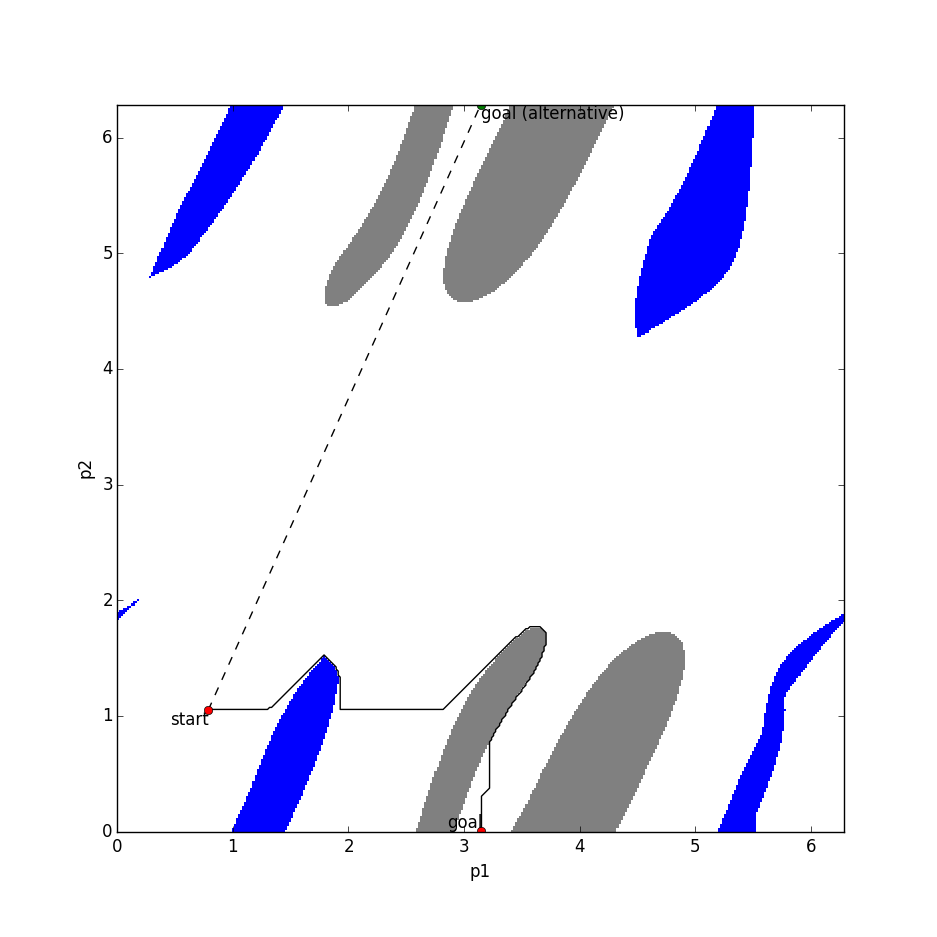
\includegraphics[width=0.7\textwidth]{figure_1.png}
    \flushleft

    In this figure, we have plotted the results of all the tasks from this assignment:

    \begin{itemize}
        \item Gray C-obstacles correspond to the obstacles $o_1$ and $o_2$.
        \item Blue C-obstacles correspond to the obstacles $o_3$ and $o_4$.
        \item We have plotted the point-sized manipulator configurations ``start'' and ``goal'', as
            well as the path between them (using our A* pathfinding algorithm).
        \item We have plotted an alternative goal under the assumption that our joints can rotate
            over the $2\pi$ boundary, hence wrapping around the plotted space. This leads us to
            a simpler path (dashed) between ``start'' and ``goal (alternative)'' without obstructions.
    \end{itemize}

    
	    	
\end {enumerate}
\end{document}
